%----------------------------------------------------------------------------
%----------------------------------------------------------------------------
%				    	SETUP
%----------------------------------------------------------------------------
%----------------------------------------------------------------------------

\documentclass[11pt]{article}

%----------------------------------------------------------------------------
%			  	   PACKAGES
%----------------------------------------------------------------------------

%%%%%%%%%%%%%%%%%%%%%%%
% 	  Packages
%%%%%%%%%%%%%%%%%%%%%%%

%% Fonts and Symbols
%% --------------------------
\usepackage{
	amsmath,			% math operators
	amssymb,			% math symbols
	courier,			% better tt font for listings
	soul,				% strike through with \st{}
	url,				% embed urls in text
	xcolor,				% color!
%	xfrac,				% fancy fractions
}

% preserve default font for URLs
\renewcommand*{\UrlFont}{\rmfamily}

%% Graphics
%% --------------------
\usepackage{
	graphicx,			% allows insertion of images
	subfigure,			% allows subfigures (a), (b), etc.
}
\graphicspath{ {graphics/} }	% (graphicx) relative path to graphics folder

%% Tables
%% --------------------------
\usepackage{
	booktabs,			% better tables, discourages vertical rulings
	multicol,			% allow multi columns
}

%% Layout Alteration
%% --------------------------
\usepackage{
%	caption,			% line breaks in captions with \\
%	changepage,			% change margins for PARTS of pages with (adjustwidth)
	geometry,			% change the margins for specific PAGES
	parskip,			% disable indents
	rotating,			% sideways figures
	setspace,			% single, double spacing
}
\geometry{				% specify page size options for (geometry)
	a4paper, 			% paper size
	hmargin=1in,		% horizontal margins
	vmargin=1in,		% vertical margins
}


%% Units
%% --------------------------
\usepackage{
	siunitx,			% has S (decimal align) column type
}
% Include peak-to-peak voltage unit
\DeclareSIUnit[]\voltpp
{V_{pp}}

\sisetup{input-symbols = {()},  % do not treat "(" and ")" in any special way
group-digits  = false, 	% no grouping of digits
%	load-configurations = abbreviations,
%	per-mode = symbol,
}

%% Misc
%% --------------------------
\usepackage{
	enumitem,			% better control of enumerations, descriptions, etc
%	pdfpages,			% include external pdfs
}

%% References
%% --------------------------
\usepackage[backend=biber,style=ieee]{biblatex}
\addbibresource{ELEC300_Lab_03.bib}

%----------------------------------------------------------------------------
%		     MACROS AND COMMANDS
%----------------------------------------------------------------------------

% Defines a new command for the horizontal lines, change thickness here
\newcommand{\HRule}{\rule{\linewidth}{0.5mm}}

% override S column type with centered text column
\newcommand{\textcol}[1]{\multicolumn{1}{c}{#1}}


%----------------------------------------------------------------------------
%----------------------------------------------------------------------------
%				   DOCUMENT
%----------------------------------------------------------------------------
%----------------------------------------------------------------------------

\begin{document}

\doublespacing
\begin{center}
	\begin{LARGE}
		Department of Electrical and Computer Engineering \\
		University of Victoria \\
		ELEC 300 - Linear Circuits II \\[1cm]
		\textsc{Laboratory Report}
		\\[1cm]
	\end{LARGE}
\end{center}

\begin{tabular}{ p{0.25\textwidth} p{0.75\textwidth} }
	Experiment No.: & 2 \\ 
	Title: & Frequency response of linear systems \\ 
	Date of experiment:& 19 February, 2016 \\ 
	& \\
	Report submitted on:& 26 February, 2016 \\ 
	To: & TA, B07 \\ 
	& \\
	Names: & M. Drinnan (V00755525)\\
	& T. Mulligan (V00819591) \\
	& T. Stephen (V00812021) 
\end{tabular}

\newpage
\section{Objective}\label{sec:objective}
Short summary of the experiment and results obtained.

\section{Introduction}\label{sec:intro}

\begin{equation}\label{eq:tf}
	H \left( s \right) = K { s - z \over s - p }
\end{equation}

\begin{figure}[tbph]
\centering
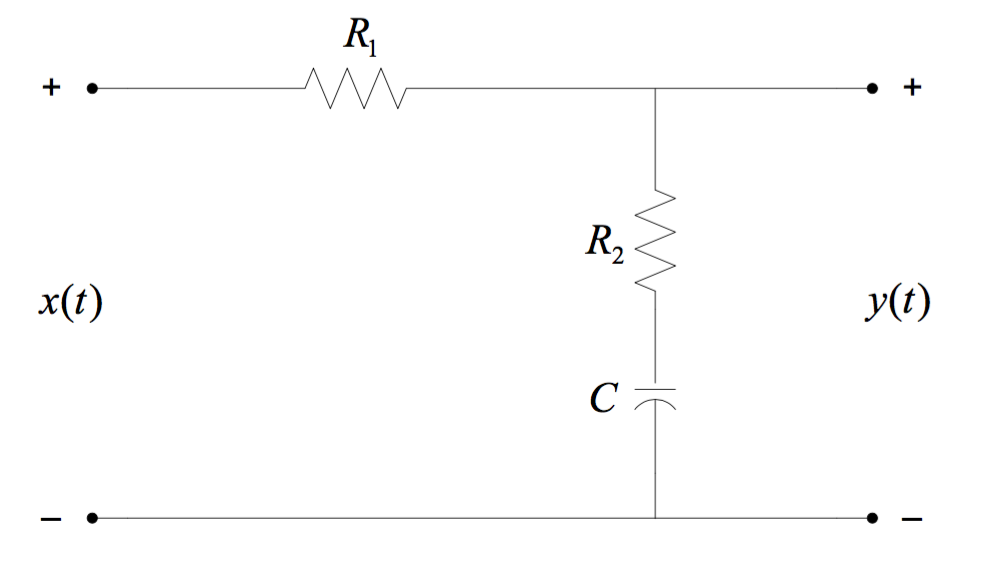
\includegraphics[width=0.7\linewidth]{graphics/lag-schematic}
\caption{Schematic of a phase lag circuit}
\label{fig:schematic}
\end{figure}
For the circuit in Fig. \ref{fig:schematic}, the transfer function is:
\begin{equation}\label{eq:tf-phaselag}
H \left( s \right) = { R_2 + \frac{1}{sC} \over R_1 + R_2 + \frac{1}{sC}} = {R_2 \over R_1 + R_2 } { s + \frac{1}{C R_2} \over s + \frac{1}{C \left( R_1 + R_2 \right)} }.
\end{equation}
Comparing \eqref{eq:tf} with \eqref{eq:tf-phaselag} gives:
\begin{align*}
K &= {R_2 \over R_1 + R_2 } \\
\left|z\right| &= \frac{1}{C R_2} \\
\left|p\right| &= \frac{1}{C \left( R_1 + R_2 \right)}.
\end{align*}

\section{Results and Discussion}\label{sec:results-and-discussion}
Fig.~\ref{fig:schematic} was realized with damping factor $\zeta = 0.1$.
Using \eqref{eqn:damping}, $R_a = \SI{70.2}{\kilo\ohm}$.
The opamp supply power was set at \SI{+-15}{\volt}.
An input signal of 1 $\si{\volt}_{pp}$ at \SI{50}{\hertz} square wave was applied to the circuit.
One pulse of the square wave will behave locally like a unit step function.

The output of this circuit is shown in Fig.~\ref{fig:overshoot}.
The large overshoot corresponds to significant underdamping, which is consistent with $\zeta = 0.1$.

\pagebreak

\begin{figure}[tbph]
	\centering
	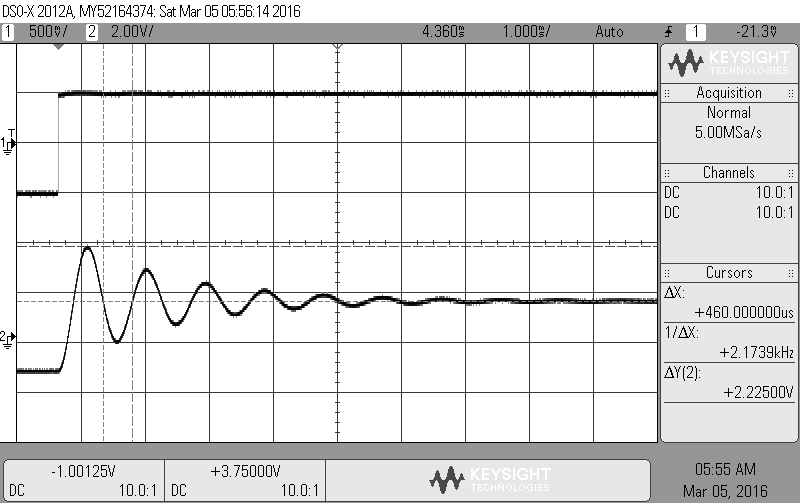
\includegraphics[width=0.7\linewidth]{graphics/overshoot}
	\caption{Measured response of second order system}
	\label{fig:overshoot}
\end{figure}

The measured values are $O_v = \SI{2.225}{\volt}$ and $T_p = \SI{460}{\micro\second}$.
As the transient response is damped, the value of the output settles to \SI{2.8}{\volt}.
This is consistent with $G = 1.8$.

\section{Conclusion}\label{sec:conclusion}
Our results confirm a sinusoid is negatively shifted by a capacitor, as well as the low-pass filter nature of the voltage across a capacitor: when the frequency of the sinusoid across the capacitor the capacitor is low it acts similar to an open circuit, and when the frequency is high the capacitor acts like a short circuit.
The negative phase shift behaviour of a capacitor justifies the circuit's \textit{phase lag} denomination.


\newpage
\printbibliography[heading=bibintoc,title={References}]

\end{document}
